% Created by tikzDevice version 0.10.1 on 2018-06-14 11:50:00
% !TEX encoding = UTF-8 Unicode
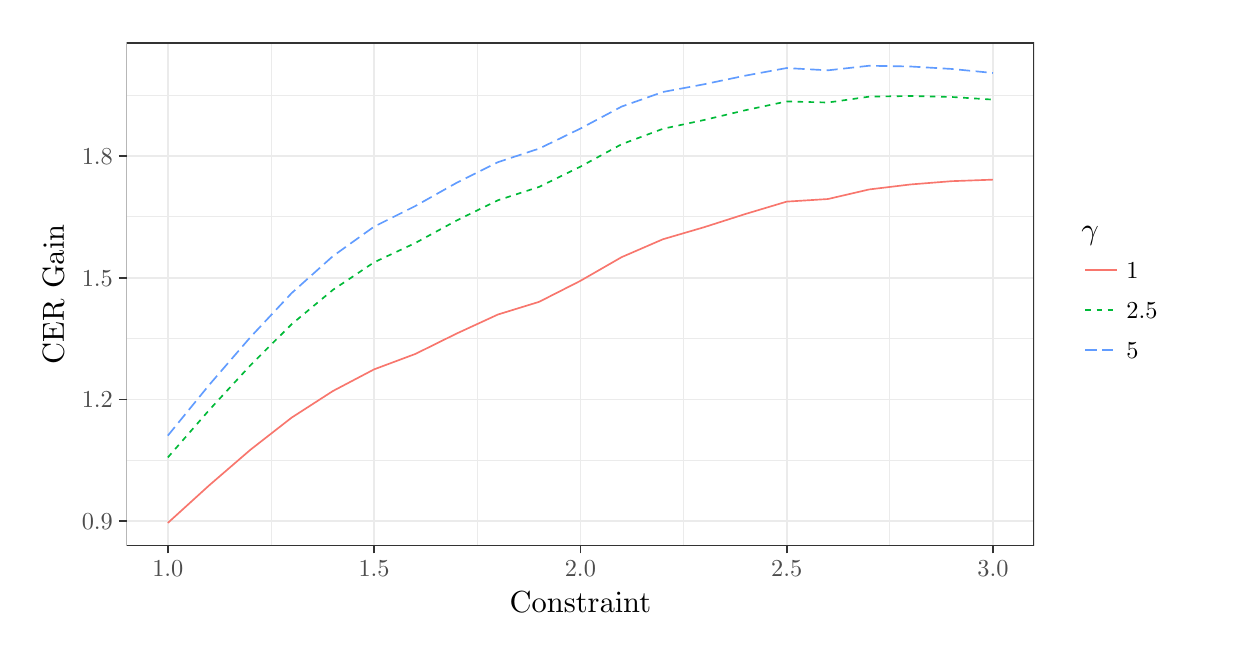
\begin{tikzpicture}[x=1pt,y=1pt]
\definecolor{fillColor}{RGB}{255,255,255}
\path[use as bounding box,fill=fillColor,fill opacity=0.00] (0,0) rectangle (426.79,216.81);
\begin{scope}
\path[clip] (  0.00,  0.00) rectangle (426.79,216.81);
\definecolor{drawColor}{RGB}{255,255,255}
\definecolor{fillColor}{RGB}{255,255,255}

\path[draw=drawColor,line width= 0.6pt,line join=round,line cap=round,fill=fillColor] (  0.00,  0.00) rectangle (426.79,216.81);
\end{scope}
\begin{scope}
\path[clip] ( 35.74, 29.59) rectangle (363.70,211.31);
\definecolor{fillColor}{RGB}{255,255,255}

\path[fill=fillColor] ( 35.74, 29.59) rectangle (363.70,211.31);
\definecolor{drawColor}{gray}{0.92}

\path[draw=drawColor,line width= 0.3pt,line join=round] ( 35.74, 60.51) --
	(363.70, 60.51);

\path[draw=drawColor,line width= 0.3pt,line join=round] ( 35.74,104.47) --
	(363.70,104.47);

\path[draw=drawColor,line width= 0.3pt,line join=round] ( 35.74,148.43) --
	(363.70,148.43);

\path[draw=drawColor,line width= 0.3pt,line join=round] ( 35.74,192.39) --
	(363.70,192.39);

\path[draw=drawColor,line width= 0.3pt,line join=round] ( 87.92, 29.59) --
	( 87.92,211.31);

\path[draw=drawColor,line width= 0.3pt,line join=round] (162.45, 29.59) --
	(162.45,211.31);

\path[draw=drawColor,line width= 0.3pt,line join=round] (236.99, 29.59) --
	(236.99,211.31);

\path[draw=drawColor,line width= 0.3pt,line join=round] (311.53, 29.59) --
	(311.53,211.31);

\path[draw=drawColor,line width= 0.6pt,line join=round] ( 35.74, 38.53) --
	(363.70, 38.53);

\path[draw=drawColor,line width= 0.6pt,line join=round] ( 35.74, 82.49) --
	(363.70, 82.49);

\path[draw=drawColor,line width= 0.6pt,line join=round] ( 35.74,126.45) --
	(363.70,126.45);

\path[draw=drawColor,line width= 0.6pt,line join=round] ( 35.74,170.41) --
	(363.70,170.41);

\path[draw=drawColor,line width= 0.6pt,line join=round] ( 50.65, 29.59) --
	( 50.65,211.31);

\path[draw=drawColor,line width= 0.6pt,line join=round] (125.18, 29.59) --
	(125.18,211.31);

\path[draw=drawColor,line width= 0.6pt,line join=round] (199.72, 29.59) --
	(199.72,211.31);

\path[draw=drawColor,line width= 0.6pt,line join=round] (274.26, 29.59) --
	(274.26,211.31);

\path[draw=drawColor,line width= 0.6pt,line join=round] (348.80, 29.59) --
	(348.80,211.31);
\definecolor{drawColor}{RGB}{248,118,109}

\path[draw=drawColor,line width= 0.6pt,line join=round] ( 50.65, 37.85) --
	( 65.55, 51.39) --
	( 80.46, 64.26) --
	( 95.37, 75.89) --
	(110.28, 85.50) --
	(125.18, 93.34) --
	(140.09, 98.91) --
	(155.00,106.28) --
	(169.91,113.15) --
	(184.81,117.74) --
	(199.72,125.32) --
	(214.63,133.89) --
	(229.54,140.35) --
	(244.44,144.71) --
	(259.35,149.48) --
	(274.26,153.95) --
	(289.17,154.89) --
	(304.07,158.35) --
	(318.98,160.15) --
	(333.89,161.34) --
	(348.80,161.89);
\definecolor{drawColor}{RGB}{0,186,56}

\path[draw=drawColor,line width= 0.6pt,dash pattern=on 2pt off 2pt ,line join=round] ( 50.65, 61.51) --
	( 65.55, 78.60) --
	( 80.46, 94.77) --
	( 95.37,109.64) --
	(110.28,122.05) --
	(125.18,132.02) --
	(140.09,139.01) --
	(155.00,147.13) --
	(169.91,154.44) --
	(184.81,159.27) --
	(199.72,166.59) --
	(214.63,174.70) --
	(229.54,180.27) --
	(244.44,183.45) --
	(259.35,186.98) --
	(274.26,190.15) --
	(289.17,189.76) --
	(304.07,191.88) --
	(318.98,192.12) --
	(333.89,191.76) --
	(348.80,190.81);
\definecolor{drawColor}{RGB}{97,156,255}

\path[draw=drawColor,line width= 0.6pt,dash pattern=on 4pt off 2pt ,line join=round] ( 50.65, 69.40) --
	( 65.55, 87.67) --
	( 80.46,104.94) --
	( 95.37,120.88) --
	(110.28,134.24) --
	(125.18,144.91) --
	(140.09,152.37) --
	(155.00,160.75) --
	(169.91,168.21) --
	(184.81,173.11) --
	(199.72,180.35) --
	(214.63,188.30) --
	(229.54,193.57) --
	(244.44,196.36) --
	(259.35,199.48) --
	(274.26,202.22) --
	(289.17,201.39) --
	(304.07,203.05) --
	(318.98,202.78) --
	(333.89,201.89) --
	(348.80,200.44);
\definecolor{drawColor}{gray}{0.20}

\path[draw=drawColor,line width= 0.6pt,line join=round,line cap=round] ( 35.74, 29.59) rectangle (363.70,211.31);
\end{scope}
\begin{scope}
\path[clip] (  0.00,  0.00) rectangle (426.79,216.81);
\definecolor{drawColor}{gray}{0.30}

\node[text=drawColor,anchor=base east,inner sep=0pt, outer sep=0pt, scale=  0.88] at ( 30.79, 35.50) {0.9};

\node[text=drawColor,anchor=base east,inner sep=0pt, outer sep=0pt, scale=  0.88] at ( 30.79, 79.46) {1.2};

\node[text=drawColor,anchor=base east,inner sep=0pt, outer sep=0pt, scale=  0.88] at ( 30.79,123.42) {1.5};

\node[text=drawColor,anchor=base east,inner sep=0pt, outer sep=0pt, scale=  0.88] at ( 30.79,167.38) {1.8};
\end{scope}
\begin{scope}
\path[clip] (  0.00,  0.00) rectangle (426.79,216.81);
\definecolor{drawColor}{gray}{0.20}

\path[draw=drawColor,line width= 0.6pt,line join=round] ( 32.99, 38.53) --
	( 35.74, 38.53);

\path[draw=drawColor,line width= 0.6pt,line join=round] ( 32.99, 82.49) --
	( 35.74, 82.49);

\path[draw=drawColor,line width= 0.6pt,line join=round] ( 32.99,126.45) --
	( 35.74,126.45);

\path[draw=drawColor,line width= 0.6pt,line join=round] ( 32.99,170.41) --
	( 35.74,170.41);
\end{scope}
\begin{scope}
\path[clip] (  0.00,  0.00) rectangle (426.79,216.81);
\definecolor{drawColor}{gray}{0.20}

\path[draw=drawColor,line width= 0.6pt,line join=round] ( 50.65, 26.84) --
	( 50.65, 29.59);

\path[draw=drawColor,line width= 0.6pt,line join=round] (125.18, 26.84) --
	(125.18, 29.59);

\path[draw=drawColor,line width= 0.6pt,line join=round] (199.72, 26.84) --
	(199.72, 29.59);

\path[draw=drawColor,line width= 0.6pt,line join=round] (274.26, 26.84) --
	(274.26, 29.59);

\path[draw=drawColor,line width= 0.6pt,line join=round] (348.80, 26.84) --
	(348.80, 29.59);
\end{scope}
\begin{scope}
\path[clip] (  0.00,  0.00) rectangle (426.79,216.81);
\definecolor{drawColor}{gray}{0.30}

\node[text=drawColor,anchor=base,inner sep=0pt, outer sep=0pt, scale=  0.88] at ( 50.65, 18.58) {1.0};

\node[text=drawColor,anchor=base,inner sep=0pt, outer sep=0pt, scale=  0.88] at (125.18, 18.58) {1.5};

\node[text=drawColor,anchor=base,inner sep=0pt, outer sep=0pt, scale=  0.88] at (199.72, 18.58) {2.0};

\node[text=drawColor,anchor=base,inner sep=0pt, outer sep=0pt, scale=  0.88] at (274.26, 18.58) {2.5};

\node[text=drawColor,anchor=base,inner sep=0pt, outer sep=0pt, scale=  0.88] at (348.80, 18.58) {3.0};
\end{scope}
\begin{scope}
\path[clip] (  0.00,  0.00) rectangle (426.79,216.81);
\definecolor{drawColor}{RGB}{0,0,0}

\node[text=drawColor,anchor=base,inner sep=0pt, outer sep=0pt, scale=  1.10] at (199.72,  5.50) {Constraint};
\end{scope}
\begin{scope}
\path[clip] (  0.00,  0.00) rectangle (426.79,216.81);
\definecolor{drawColor}{RGB}{0,0,0}

\node[text=drawColor,rotate= 90.00,anchor=base,inner sep=0pt, outer sep=0pt, scale=  1.10] at ( 13.08,120.45) {CER Gain};
\end{scope}
\begin{scope}
\path[clip] (  0.00,  0.00) rectangle (426.79,216.81);
\definecolor{fillColor}{RGB}{255,255,255}

\path[fill=fillColor] (375.09, 87.48) rectangle (421.29,153.41);
\end{scope}
\begin{scope}
\path[clip] (  0.00,  0.00) rectangle (426.79,216.81);
\definecolor{drawColor}{RGB}{0,0,0}

\node[text=drawColor,anchor=base west,inner sep=0pt, outer sep=0pt, scale=  1.10] at (380.78,140.15) {$\gamma$};
\end{scope}
\begin{scope}
\path[clip] (  0.00,  0.00) rectangle (426.79,216.81);
\definecolor{fillColor}{RGB}{255,255,255}

\path[fill=fillColor] (380.78,122.08) rectangle (395.23,136.53);
\end{scope}
\begin{scope}
\path[clip] (  0.00,  0.00) rectangle (426.79,216.81);
\definecolor{drawColor}{RGB}{248,118,109}

\path[draw=drawColor,line width= 0.6pt,line join=round] (382.22,129.31) -- (393.78,129.31);
\end{scope}
\begin{scope}
\path[clip] (  0.00,  0.00) rectangle (426.79,216.81);
\definecolor{fillColor}{RGB}{255,255,255}

\path[fill=fillColor] (380.78,107.63) rectangle (395.23,122.08);
\end{scope}
\begin{scope}
\path[clip] (  0.00,  0.00) rectangle (426.79,216.81);
\definecolor{drawColor}{RGB}{0,186,56}

\path[draw=drawColor,line width= 0.6pt,dash pattern=on 2pt off 2pt ,line join=round] (382.22,114.85) -- (393.78,114.85);
\end{scope}
\begin{scope}
\path[clip] (  0.00,  0.00) rectangle (426.79,216.81);
\definecolor{fillColor}{RGB}{255,255,255}

\path[fill=fillColor] (380.78, 93.17) rectangle (395.23,107.63);
\end{scope}
\begin{scope}
\path[clip] (  0.00,  0.00) rectangle (426.79,216.81);
\definecolor{drawColor}{RGB}{97,156,255}

\path[draw=drawColor,line width= 0.6pt,dash pattern=on 4pt off 2pt ,line join=round] (382.22,100.40) -- (393.78,100.40);
\end{scope}
\begin{scope}
\path[clip] (  0.00,  0.00) rectangle (426.79,216.81);
\definecolor{drawColor}{RGB}{0,0,0}

\node[text=drawColor,anchor=base west,inner sep=0pt, outer sep=0pt, scale=  0.88] at (397.04,126.28) {1};
\end{scope}
\begin{scope}
\path[clip] (  0.00,  0.00) rectangle (426.79,216.81);
\definecolor{drawColor}{RGB}{0,0,0}

\node[text=drawColor,anchor=base west,inner sep=0pt, outer sep=0pt, scale=  0.88] at (397.04,111.82) {2.5};
\end{scope}
\begin{scope}
\path[clip] (  0.00,  0.00) rectangle (426.79,216.81);
\definecolor{drawColor}{RGB}{0,0,0}

\node[text=drawColor,anchor=base west,inner sep=0pt, outer sep=0pt, scale=  0.88] at (397.04, 97.37) {5};
\end{scope}
\end{tikzpicture}
